\documentclass[12pt,letterpaper]{exam}
\usepackage[lmargin=1in,rmargin=1in,tmargin=1in,bmargin=1in]{geometry}
\usepackage{../style/exams}

% -------------------
% Course & Exam Information
% -------------------
\newcommand{\course}{MAT 101: Exam 1}
\newcommand{\term}{Summer -- 2022}
\newcommand{\examdate}{05/26/2022}
\newcommand{\timelimit}{85 Minutes}

\setbool{hideans}{false} % Student: True; Instructor: False

% -------------------
% Content
% -------------------
\begin{document}

\examtitle
\instructions{Write your name on the appropriate line on the exam cover sheet. This exam contains \numpages\ pages (including this cover page) and \numquestions\ questions. Check that you have every page of the exam. Answer the questions in the spaces provided on the question sheets. Be sure to answer every part of each question and show all your work.} 
\scores
%\bottomline
\newpage

% ---------
% Questions
% ---------
\begin{questions}

% Question 1
\newpage
\question[10] For each of the following numbers, indicate with a checkmark whether each of the numbers is a natural, integer, rational, irrational, real, or complex number. 
        \begin{table}[!ht]
        \centering
        \begin{tabular}{rcccccc}
         & Natural & Integer & Rational & Irrational & Real & Complex \\[0.3cm]
        $13$ & \usol{0.5cm}{\cmark} & \usol{0.5cm}{\cmark} & \usol{0.5cm}{\cmark} & \uans{1.3cm} & \usol{0.5cm}{\cmark} & \usol{0.5cm}{\cmark} \\[0.3cm]
        $0$ & \uans{1.3cm} & \usol{0.5cm}{\cmark} & \usol{0.5cm}{\cmark} & \uans{1.3cm} & \usol{0.5cm}{\cmark} & \usol{0.5cm}{\cmark} \\[0.3cm]
        $-7$ & \uans{1.3cm} & \usol{0.5cm}{\cmark} & \usol{0.5cm}{\cmark} & \uans{1.3cm} & \usol{0.5cm}{\cmark} & \usol{0.5cm}{\cmark} \\[0.3cm]
        $34/4$ & \uans{1.3cm} & \uans{1.3cm} & \usol{0.5cm}{\cmark} & \uans{1.3cm} & \usol{0.5cm}{\cmark} & \usol{0.5cm}{\cmark} \\[0.3cm]
	$0.\overline{13}$ & \uans{1.3cm} & \uans{1.3cm} & \usol{0.5cm}{\cmark} & \uans{1.3cm} & \usol{0.5cm}{\cmark} & \usol{0.5cm}{\cmark} \\[0.3cm]
        $5/7$ & \uans{1.3cm} & \uans{1.3cm} & \usol{0.5cm}{\cmark} & \uans{1.3cm} & \usol{0.5cm}{\cmark} & \usol{0.5cm}{\cmark} \\[0.3cm]
        $-5.78$ & \uans{1.3cm} & \uans{1.3cm} & \usol{0.5cm}{\cmark} & \uans{1.3cm} & \usol{0.5cm}{\cmark} & \usol{0.5cm}{\cmark} \\[0.3cm]
        $\sqrt{49}$ & \usol{0.5cm}{\cmark} & \usol{0.5cm}{\cmark} & \usol{0.5cm}{\cmark} & \uans{1.3cm} & \usol{0.5cm}{\cmark} & \usol{0.5cm}{\cmark} \\[0.3cm]
        $\pi$ & \uans{1.3cm} & \uans{1.3cm} & \uans{1.3cm} & \usol{0.5cm}{\cmark} & \usol{0.5cm}{\cmark} & \usol{0.5cm}{\cmark} \\[0.3cm]
        $\sqrt{-4}$ & \uans{1.3cm} & \uans{1.3cm} & \uans{1.3cm} & \uans{1.3cm} & \uans{1.3cm} & \usol{0.5cm}{\cmark} 
        \end{tabular}
        \end{table}



% Question 2
\newpage
\question[10] Find the prime factorizations for each of the following integers:
        \begin{enumerate}[(a)]
        \item 29
        \item 84
        \item 495
        \end{enumerate} \pspace

\sol 
\begin{enumerate}[(a)]
\item $29= 29^1$ \pspace
        
\item $84= 2^2 \cdot 3 \cdot 7$
        	\[
        	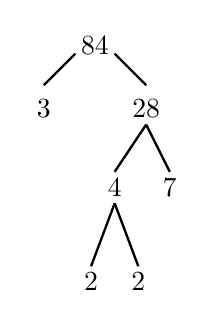
\begin{tikzpicture}
        	\node at (-0.15,0) {$84$};
        	\draw[line width=0.03cm] (-0.4,-0.1) -- (-0.8,-0.5);
        	\node at (-0.8,-0.8) {$3$};
        	\draw[line width=0.03cm]  (0.1,-0.1) -- (0.5,-0.5);
        	\node at (0.5,-0.8) {$28$};
        	
        	\draw[line width=0.03cm] (0.5,-1) -- (0.1,-1.6);
        	\node at (0.1,-1.8) {$4$};
        	\draw[line width=0.03cm] (0.5,-1) -- (0.8,-1.6);
        	\node at (0.8,-1.8) {$7$};
		
        	\draw[line width=0.03cm] (0.4,-2.8) -- (0.1,-2);
        	\node at (0.4,-3.0) {$2$};
	\draw[line width=0.03cm] (-0.2,-2.8) -- (0.1,-2);
        	\node at (-0.2,-3.0) {$2$};		
        	\end{tikzpicture}
        	\] \pspace
	
\item $495= 3^2 \cdot 5 \cdot 11$
        	\[
        	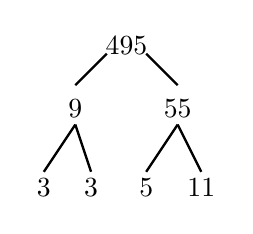
\begin{tikzpicture}
        	\node at (-0.15,0) {$495$};
        	\draw[line width=0.03cm] (-0.4,-0.1) -- (-0.8,-0.5);
        	\node at (-0.8,-0.8) {$9$};
        	\draw[line width=0.03cm]  (0.1,-0.1) -- (0.5,-0.5);
        	\node at (0.5,-0.8) {$55$};
        		
        	\draw[line width=0.03cm] (-0.8,-1) -- (-1.2,-1.6);
        	\node at (-1.2,-1.8) {$3$};
        	\draw[line width=0.03cm] (-0.8,-1) -- (-0.6,-1.6);
        	\node at (-0.6,-1.8) {$3$};
        	
        	\draw[line width=0.03cm] (0.5,-1) -- (0.1,-1.6);
        	\node at (0.1,-1.8) {$5$};
        	\draw[line width=0.03cm] (0.5,-1) -- (0.8,-1.6);
        	\node at (0.8,-1.8) {$11$};
        	\end{tikzpicture}
        	\]
\end{enumerate}



% Question 3
\newpage
\question[10] Using an argument involving the square root, show that the integer 109 is prime. \pspace

{\itshape If a number $n$ is composite, then it has a prime factor between 2 and $\sqrt{n}$. We know that $\sqrt{109} \approx 10.4403$. Therefore, if 109 is composite then one of the primes 2, 3, 5, or 7 must be a factor of 109. \pspace

Because 109 is not even, it is not divisible by 2. The sum of the digits of 109 is 10, which is not divisible by 3 so that 109 is not divisible by 3. Because 109 does not end in a 0 or 5, 109 is not divisible by 5. Finally, we can check that $109/7 \approx 15.5714$ so that 109 is not divisible by 7. [One can also use the fact that $109/2 \approx 54.5$, $109/3 \approx 36.3333$, and $109/5 \approx 21.8$ so that 109 is not divisible by 2, 3, or 5, respectively.] \pspace

But then 109 cannot be composite. Therefore, 109 is prime. 
}



% Question 4
\newpage
\question[10] Showing all your work, compute the following:
	\begin{enumerate}[(a)]
	\item $\gcd(50, 66)$
	\item $\lcm(14, 22)$
	\item $\gcd(2^{12} \cdot 3^{40} \cdot 7^{12} \cdot 13^{70}, 2^{30} \cdot 3^{28} \cdot 5^{46} \cdot 11^{90})$
	\item $\lcm(2^{12} \cdot 3^{40} \cdot 7^{12} \cdot 13^{70}, 2^{30} \cdot 3^{28} \cdot 5^{46} \cdot 11^{90})$
	\end{enumerate} \pspace

\sol
\begin{enumerate}[(a)]
\item $\gcd(50, 66)= \gcd(2 \cdot 5^2, 2 \cdot 3 \cdot 11)= 2$ \pspace

\item $\lcm(14, 22)= \lcm(2 \cdot 7, 2 \cdot 11)= 2 \cdot 7 \cdot 11= 154$ \pspace

\item $\gcd(2^{12} \cdot 3^{40} \cdot 7^{12} \cdot 13^{70}, 2^{30} \cdot 3^{28} \cdot 5^{46} \cdot 11^{90})= 2^{12} \cdot 3^{28}$ \pspace

\item $\lcm(2^{12} \cdot 3^{40} \cdot 7^{12} \cdot 13^{70}, 2^{30} \cdot 3^{28} \cdot 5^{46} \cdot 11^{90})= 2^{30} \cdot 3^{40} \cdot 5^{46} \cdot 7^{12} \cdot 11^{90} \cdot 13^{70}$
\end{enumerate}



% Question 5
\newpage
\question[10] Showing all your work, reduce the following rational numbers completely:
	\begin{enumerate}[(a)]
	\item $\dfrac{21}{45}$
	\item $\dfrac{7}{22}$
	\item $\dfrac{132}{30}$
	\end{enumerate} \pspace

\sol
\begin{enumerate}[(a)]
\item $\dfrac{21}{45}= \dfrac{3 \cdot 7}{3^2 \cdot 5}= \dfrac{\cancel{3} \cdot 7}{3^{\cancel{2}^1} \cdot 5}= \dfrac{7}{15}$ \pspace

\item $\dfrac{7}{22}= \dfrac{7}{22}$ \pspace

\item $\dfrac{132}{30}= \dfrac{2^2 \cdot 3 \cdot 11}{2 \cdot 3 \cdot 5}= \dfrac{2^{\cancel{2}^1} \cdot \cancel{3} \cdot 11}{\cancel{2} \cdot \cancel{3} \cdot 5}= \dfrac{22}{5}$
\end{enumerate}



% Question 6
\newpage
\question[10] Showing all your work and being sure to simplify as much as possible, compute the following:
	\begin{enumerate}[(a)] \itemsep=0.3cm
	\item $\dfrac{5}{7} - \dfrac{8}{21}$
	\item $\dfrac{9}{8} + \dfrac{7}{12}$
	\item $\dfrac{20}{99} \cdot \dfrac{21}{10}$
	\item $\dfrac{\;\;\dfrac{26}{15}\;\;}{\;\;\dfrac{20}{9}\;\;}$
	\end{enumerate} \pspace

\sol
\begin{enumerate}[(a)]
\item $\dfrac{5}{7} - \dfrac{8}{21}= \dfrac{15}{21} - \dfrac{8}{21}= \dfrac{15 - 8}{21}= \dfrac{7}{21}= \dfrac{1}{3}$ \pspace

\item $\dfrac{9}{8} + \dfrac{7}{12}= \dfrac{27}{24} + \dfrac{14}{24}= \dfrac{27 + 14}{24}= \dfrac{41}{24}$ \pspace

\item $\dfrac{20}{99} \cdot \dfrac{21}{10}= \dfrac{2^2 \cdot 5}{3^2 \cdot 11} \cdot \dfrac{3 \cdot 7}{2 \cdot 5}= \dfrac{2^{\cancel{2}^1} \cdot \cancel{5}}{3^{\cancel{2}^1} \cdot 11} \cdot \dfrac{\cancel{3} \cdot 7}{\cancel{2} \cdot \cancel{5}}= \dfrac{14}{33}$ \pspace

\item $\dfrac{\;\;\dfrac{26}{15}\;\;}{\;\;\dfrac{20}{9}\;\;}= \dfrac{26}{15} \cdot \dfrac{9}{20}= \dfrac{\cancel{2} \cdot 13}{\cancel{3} \cdot 5} \cdot \dfrac{3^{\cancel{2}^1}}{2^{\cancel{2}^1} \cdot 5}= \dfrac{39}{50}$
\end{enumerate}



% Question 7
\newpage
\question[10] Convert the following decimal numbers to a rational number, being sure to simplify as much as possible:
	\begin{enumerate}[(a)]
	\item $0.240$
	\item $0.\overline{18}$
	\end{enumerate} \pspace

\sol
\begin{enumerate}[(a)]
\item $0.240= \dfrac{240}{1000}= \dfrac{24 \cdot 10}{100 \cdot 10}= \dfrac{24}{100}= \dfrac{6}{25}$ \pspace

\item \phantom{.} \par
	\begin{table}[!ht]
	\centering\small
	\begin{tabular}{rccc}
	& $100N$ & $=$ & $18.18181818\overline{18}$ \\ 
	$-$ & $N$ & $=$ & $\phantom{1}0.18181818\overline{18}$ \\ \hline
	& $99N$ & $=$ & $18$ \\[0.1cm]
	& $N$ & $=$ & $\frac{18}{99}$ \\[0.1cm]
	& $N$ & $=$ & $\frac{2}{11}$
	\end{tabular}
	\end{table} \par

	\[
	0.\overline{18}= \dfrac{2}{11}
	\] 
\end{enumerate}



% Question 8
\newpage
\question[10] Write the following numbers in scientific notation:
	\begin{enumerate}[(a)]
	\item $178.3$
	\item $4.64$
	\item $0.0000091$
	\item $167000$
	\end{enumerate} \pspace

\sol
\begin{enumerate}[(a)]
\item $178.3= 1.783 \cdot 10^2$ \pspace

\item $4.64= 4.64 \cdot 10^0$ \pspace

\item $9.1 \cdot 10^{-6}$ \pspace

\item $167000= 1.67 \cdot 10^5$
\end{enumerate}



% Question 9
\newpage
\question[10] Write the following scientific numbers in ordinary decimal notation:
	\begin{enumerate}[(a)]
	\item $1.45 \cdot 10^5$ 
	\item $6.92 \cdot 10^{-3}$
	\item $-8.3 \cdot 10^0$
	\end{enumerate} \pspace

\sol
\begin{enumerate}[(a)]
\item $1.45 \cdot 10^5= 145\,000$ \pspace

\item $6.92 \cdot 10^{-3}= 0.00692$ \pspace

\item $-8.3 \cdot 10^0= -8.3$
\end{enumerate}



% Question 10
\newpage
\question[10] Simplify the follow expressions, showing all your work and using no negative powers:
	\begin{enumerate}[(a)] \itemsep=0.3cm
	\item $x^5 y^2 (xy^3)^0 (x^3y)^4$
	\item $z^4(x^5 z^3)^{-2} (x^3 y^2)^2$
	\item $\dfrac{x^{-5} y^6}{(x^3 y^{-4})^{-2}}$
	\item $\dfrac{(x^8 y^{12})^{1/4}}{\sqrt{x^4 y^5}}$
	\end{enumerate} \pspace

\sol
\begin{enumerate}[(a)]
\item $x^5 y^2 (xy^3)^0 (x^3y)^4= x^5 y^2 \cdot 1 \cdot x^{12} y^4= x^{17} y^6$ \pspace

\item $z^4(x^5 z^3)^{-2} (x^3 y^2)^2= z^4 \cdot x^{-10} z^{-6} \cdot x^6 y^4= x^{-4} y^4 z^{-2}= \dfrac{y^4}{x^4 z^2}$ \pspace

\item $\dfrac{x^{-5} y^6}{(x^3 y^{-4})^{-2}}= \dfrac{x^{-5} y^6}{x^{-6} y^8}= \dfrac{x^6 y^6}{x^5 y^8}= \dfrac{x}{y^2}$ \pspace

\item $\dfrac{(x^8 y^{12})^{1/4}}{\sqrt{x^4 y^5}}= \dfrac{x^{8/4} y^{12/4}}{(x^4 y^5)^{1/2}}= \dfrac{x^2 y^3}{x^2 y^{5/2}}= \dfrac{y^3}{y^{5/2}}= y^{3 - 5/2}= y^{1/2}= \sqrt{y}$
\end{enumerate}



% Question 11
\newpage
\question[10] Showing all your work, simplify the following as much as possible:
	\begin{enumerate}[(a)]
	\item $\sqrt{68}$
	\item $\sqrt{2^8 \cdot 3 \cdot 5^3}$
	\item $\sqrt[5]{2^{10} \cdot 3^5 \cdot 5^2 \cdot 7^6}$
	\end{enumerate} \pspace

\sol 
\begin{enumerate}[(a)]
\item $\sqrt{68}= \sqrt{2^2 \cdot 17}= 2 \sqrt{17}$ \pspace

\item $\sqrt{2^8 \cdot 3 \cdot 5^3}= \sqrt{2^8 \cdot 3 \cdot (5^2 \cdot 5)}= 2^4 \cdot 5 \sqrt{3 \cdot 5}= 80 \sqrt{15}$ \pspace

\item $\sqrt[5]{2^{10} \cdot 3^5 \cdot 5^2 \cdot 7^6}= \sqrt[5]{2^{10} \cdot 3^5 \cdot 5^2 \cdot (7^5 \cdot 7)}= 2^2 \cdot 3^1 \cdot 7^1 \sqrt[5]{5^2 \cdot 7}= 84 \sqrt[5]{175}$
\end{enumerate}



% Question 12
\newpage
\question[10] Showing all your work and simplifying as much as possible, rationalize the following:
	\begin{enumerate}[(a)] \itemsep=0.3cm
	\item $\dfrac{10}{\sqrt{5}}$
	\item $\dfrac{14}{3 - \sqrt{2}}$
	\end{enumerate} \pspace

\sol
\begin{enumerate}[(a)]
\item $\dfrac{10}{\sqrt{5}}= \dfrac{10}{\sqrt{5}} \cdot \dfrac{\sqrt{5}}{\sqrt{5}}= \dfrac{10 \sqrt{5}}{5}= 2 \sqrt{5}$ \pspace

\item $\dfrac{14}{3 - \sqrt{2}}= \dfrac{14}{3 - \sqrt{2}} \cdot \dfrac{3 + \sqrt{2}}{3 + \sqrt{2}}= \dfrac{42 + 14 \sqrt{2}}{9 + 3\sqrt{2} - 3\sqrt{2} - 2}= \dfrac{42 + 14 \sqrt{2}}{7}$
\end{enumerate}



% Question 13
\newpage
\question[10] Compute each of the following and write the result in the form $a + bi$, being sure to simplify as much as possible:
	\begin{enumerate}[(a)]
	\item $(10 - 7i) - (5 - 11i)$
	\item $(4 - 3i)(11 + 6i)$
	\item $\dfrac{1 + i}{1 - 3i}$
	\end{enumerate} \pspace

\sol
\begin{enumerate}[(a)]
\item $(10 - 7i) - (5 - 11i)= 10 - 7i - 5 + 11i= 5 + 4i$ \pspace

\item $(4 - 3i)(11 + 6i)= 44 + 24i - 33i - 18i^2= 44 - 9i - 18(-1)= 44 + 18 - 9i= 62 - 9i$ \pspace

\item $\dfrac{1 + i}{1 - 3i}= \dfrac{1 + i}{1 - 3i} \cdot \dfrac{1 + 3i}{1 + 3i}= \dfrac{1 + 3i + i + 3i^2}{1 + 3i - 3i - 9i^2}= \dfrac{1 + 4i - 3}{1 + 9}= \dfrac{-2 + 4i}{10}= -\tfrac{1}{5} + \tfrac{2}{5}\,i$
\end{enumerate}



% Question 14
\newpage
\question[10] Showing all your work, compute each of the following:
	\begin{enumerate}[(a)]
	\item 18\% of 940
	\item 88\% of 7
	\item 132\% of 65
	\end{enumerate} \pspace

\sol
\begin{enumerate}[(a)]
\item $940(0.18)= 169.2$ \pspace

\item $7(0.88)= 6.16$ \pspace

\item $65(1.32)= 85.8$ 
\end{enumerate}



% Question 15
\newpage
\question[10] Showing all your work, compute each of the following:
	\begin{enumerate}[(a)]
	\item 900 decreased by 36\%
	\item 66 increased by 45\%
	\item 19 increased by 160\%
	\end{enumerate} \pspace

\sol
\begin{enumerate}[(a)]
\item $900(1 - 0.36)= 900(0.64)= 576$ \pspace

\item $66(1 + 0.45)= 66(1.45)= 95.7$ \pspace

\item $19(1 + 1.60)= 19(2.60)= 49.4$
\end{enumerate}



% Question 16
\newpage
\question[10] A student is taking a course with the following grade components:
	\begin{table}[!ht]
	\centering
	\begin{tabular}{rr}
	Presentation & 5\% \\
	Homework & 25\% \\
	Quizzes & 15\% \\
	Midterm & 25\% \\
	Final & 30\% 
	\end{tabular}
	\end{table} \par
Suppose that the student received a 94\% on the presentation, 78\% on the midterm, and 84\% on the final. If the student had a 89\% quiz average and 92\% homework average, find the student's course average. \pspace

\sol 
	\[
	\begin{aligned}
	\text{Course Average}&= \sum \text{weight} \cdot \text{average} \\[0.3cm]
	&= 5(0.94) + 25(0.92) + 15(0.89) + 25(0.78) + 30(0.84) \\[0.3cm]
	&= 4.7 + 23 + 13.35 + 19.5 + 25.2 \\[0.3cm]
	&= 85.75
	\end{aligned}
	\]



% Question 17
\newpage
\question[10] A local college uses the following credit weights in their GPA calculations:
	\begin{table}[!ht]
	\centering
	\begin{tabular}{lr|lr}
	A & 4.0 & C+ & 2.3 \\
	A$-$ & 3.7 & C & 2.0 \\
	B+ & 3.3 & C$-$ & 1.7 \\
	B & 3.0 & D & 1.0 \\
	B$-$ & 2.7 & F & 0.0
	\end{tabular}
	\end{table} \par
Suppose that student received the following grades this semester:
	\begin{table}[!ht]
	\centering
	\begin{tabular}{lcl}
	Course & Credits & Grade \\ \hline
	German I & 3 & A$-$ \\
	Freshman Seminar & 1 & A \\
	Calculus III & 4 & A$-$ \\
	Physics I & 4 & B$-$ \\
	Cultural Anthropology & 3 & B \\
	The Soviet Empire & 3 & C+
	\end{tabular}
	\end{table} \par
Showing all your work, compute this student's semester GPA. \pspace

\sol 
	\[
	\begin{aligned}
	\text{Semester GPA}&= \dfrac{\sum \text{credit} \cdot \text{weight}}{\sum \text{credits}} \\[0.3cm]
	&= {3(3.7) + 1(4.0) + 4(3.7) + 4(2.7) + 3(3.0) + 3(2.3)}{3 + 1 + 4 + 4 + 4 + 3 + 3} \\[0.3cm]
	&= \dfrac{11.1 + 4 + 14.8 + 10.8 + 9 + 6.9}{22} \\[0.3cm]
	&= \dfrac{56.6}{22} \\[0.3cm]
	&= 2.573
	\end{aligned}
	\]



% Question 18
\newpage
\question[10] A certain drug is to be administered such that the patient gets 45~mg for every 3 pounds (lb) that a patient weighs. How many milligrams (mg) should a 165~lb patient receive? \pspace

{\itshape Comparing ratios, we have\dots \pspace
	\[
	\begin{aligned}
	\dfrac{45 \text{ mg}}{3 \text{ lb}}&= \dfrac{x}{165 \text{ lb}} \\[0.3cm]
	3x&= 7425 \\[0.3cm]
	x&= 2475
	\end{aligned}
	\] \pspace
Therefore, the patient should be given 2475~mg. 
}



% Question 19
\newpage
\question[10] Mankind has met an alien civilization. They use a unit of distance known as a `kellikarn' (kn) and a unit of time called a `starpoint' (sp). It is known 15~kn is 3.2~ft and 17~sp is 1.4~min. What is 26.1~kn/sp in miles per hour? Note that there are 5280~ft in one mile. \pspace

\sol 
	\begin{table}[!ht]
	\centering
	\begin{tabular}{c|c|c|c|c}
	26.1 kn & 3.2~ft & 1~mi & 17~sp & 60~min. \\ \hline
	1~sp 	& 15~kn & 5280~ft & 1.4~min. & 1~hr.
	\end{tabular}
	= 0.768321~mph
	\end{table}



% Question 20
\newpage
\question[10] Suppose that the average cost of land in Montana is approximately \$2,000 per acre. If one acre is 4840~yd$^2$ and 1~yard (yd) is 3~feet (ft), what is the average cost of land in Montana per square foot? \pspace

\sol
	\begin{table}[!ht]
	\centering
	\begin{tabular}{c|c|c|c}
	\$2000 & 1~acre & 1~yd & 1~yd \\ \hline
	1~acre & 4840~yd$^2$ & 3~ft & 3~ft
	\end{tabular}
	= \$0.05/ft$^2$
	\end{table}


\end{questions}
\end{document}